% /*@@
%   @file      documentation.tex
%   @date      28 April 2002
%   @author    Denis Pollney
%   @desc 
%              IDAnalyticBH users guide.
%   @enddesc 
%   @version $Header$
% @@*/

%
% FIXME: Is the non-conformal schwarzschild correct in the source
% FIXME:   code???
% FIXME: Add a reference to the quasi-isotropic Kerr coordinates?
% FIXME: What is the Cadez lapse for Misner?
% FIXME: The distance calculation (tmp1) seems wrong in the
% FIXME:   brill-lindquist code.
% FIXME: Check that figure was included for Cartoon docs.


\documentclass{article}

% Use the Cactus ThornGuide style file
% (Automatically used from Cactus distribution, if you have a 
%  thorn without the Cactus Flesh download this from the Cactus
%  homepage at www.cactuscode.org)
\usepackage{../../../../../doc/latex/cactus}

\newlength{\tableWidth} \newlength{\maxVarWidth} \newlength{\paraWidth} \newlength{\descWidth} \begin{document}

\title{Using \texttt{IDAnalyticBH}}
\author{Denis Pollney}
\date{$ $Date$ $}

\maketitle

% Do not delete next line
% START CACTUS THORNGUIDE

\begin{abstract}
The \texttt{IDAnalyticBH} thorn contains a number of initial data
sets for black-hole evolutions which can be specified analytically
as metric and extrinsic curvature components. The initial data which
is included in this thorn include single Schwarzschild and Kerr black
holes, and multiple black hole Misner and Brill-Lindquist solutions.
\end{abstract}


\section{Background}

The \texttt{IDAnalyticBH} thorn exists as a central location to place any
initial dataset for black hole evolution that can be specified
analytically in terms of the metric, $g_{ab}$, and extrinsic
curvature, $K_{ab}$.

The thorn extends the \texttt{admbase::initial\_data} parameter by
adding the following datasets:
\begin{description}
  \item[\texttt{schwarzschild}] Schwarzschild, in isotropic
  coordinates;
  \item[\texttt{kerr}] Kerr, in Boyer-Lindquist coordinates;
  \item[\texttt{misner\_bh}] 2~Misner black holes;
  \item[\texttt{multiple\_misner\_bh}] $N \ge 2$ Misner black holes;
	(Alas this code is currently broken; see the level~1
	\verb|CCTK_VWarn()| warning in \verb|src/Misner_points.c|,
	function \verb|Misner_init()|.)

  \item[\texttt{bl\_bh}] Multiple Brill-Lindquist black holes.
\end{description}
Initial data for lapse and shift can also be specified in
this thorn.\\

The Cactus grid-functions corresponding to the initial data are
inherited from the thorn \texttt{CactusEinstein/ADMBase}, along with
the conformal factor grid-function, \texttt{psi} from \texttt{CactusEinstein/StaticConformal}, and its derivatives
which are optionally set based on the value of the parameters
\texttt{admbase::metric\_type} and \texttt{staticconformal::conformal\_storage}.\\

The \texttt{IDAnalyticBH} has been written and augmented over an number of
years by many Cactus authors. These include John Baker, Steve Brandt,
Carsten Gundlach, Joan Masso, Ed Seidel, Jonathan Thornburg, and
Paul Walker.
The following sections describe each of the initial datasets
and their associated parameters in turn.

\section{Schwarzschild}

The Schwarzschild metric corresponds to a single, static, black hole.
If the Cactus metric is specified as a conformal metric (by setting
\texttt{admbase::metric\_type="yes"}), then the metric is
set using isotropic coordinates \cite{CactusEinstein_IDAnalyticBH_mtw-isotropic}:
\begin{equation}
  ds^2 = -\left(\frac{2r - M}{2r + M}\right)^2
  + \left(1 + \frac{M}{2r}\right)^4 \left(dr^2 + r^2(d\theta^2
  + \sin^2\theta d\phi^2)\right),
\end{equation}
with the Schwarzschild mass given by the single free parameter $M$.
Thus, the three metric and extrinsic curvature have the values:
\begin{eqnarray}
  \hat{g}_{ab} & = & \psi^4 \delta_{ab}, \\
  \psi & = & (1 + \frac{M}{2r}), \\
  K_{ab} & = & 0.
\end{eqnarray}

The mass is specified using the parameter
\texttt{idanalyticbh::mass}. The black hole is assumed to reside at
the origin of the grid, corresponding to the location $x=y=z=0$.\\

If the \texttt{admbase::metric\_type} parameter has been set to {\tt static conformal}, then
the metric grid-functions (\texttt{admbase::gxx}, $\ldots$,
\texttt{admbase::gzz}) are given as $\delta_{ab}$, and the conformal
factor \texttt{staticconformal::psi} is set to the value specified
above. The derivatives of the conformal factor
(\texttt{staticconformal::psix}, etc.) are determined analytically.

In order to give the lapse an initial profile which corresponds to
isotropic lapse of the $4$-metric specified above, use the parameter
\begin{verbatim}
  admbase::initial_lapse = "schwarz"
\end{verbatim}
This will cause the \texttt{admbase::alp} grid-function to be
initialised to the value:
\begin{equation}
  \alpha = \frac{2r - M}{2r + M}.
\end{equation}


Note that the Schwarzschild data has the following non-standard
behaviour in response to the \texttt{admbase::metric\_type}
parameter. If the \emph{physical} metric is requested
(ie. \texttt{metric\_type} is set to \texttt{"physical"}) then a
\emph{different} form of the Schwarzschild metric is set:
Schwarzschild coordinates are set instead of the isotropic
coordinates:
\begin{equation}
  g_{xx} = g_{yy} = g_{zz} = 1 + 2M/r.
\end{equation}


In order to carry out an evolution of a single Schwarzschild
black hole of mass $m=1$, using an initial lapse of $\alpha=1$, you
could modify your parameter file as follows:

\begin{verbatim}
  ActiveThorns = "... ADMBase StaticConformal IDAnalyticBH ..."

  admbase::metric_type = "static conformal"

  admbase::initial_data = "schwarzschild"
  admbase::initial_lapse = "one"            # or "schwarz" for isotropic lapse

  idanalyticbh::mass = 1.0
\end{verbatim}


\section{Kerr}

Kerr initial data for an isolated rotating black hole is specified
using the ``quasi-isotropic'' coordinates \cite{CactusEinstein_IDAnalyticBH_brandt-seidel:1996}:
\begin{equation}
  ds^2 = \psi^4 (dr^2 + r^2(d\theta^2 + \chi^2\sin^2\theta d\phi^2)),
\end{equation}
where
\begin{eqnarray}
  \psi^4 & = & - 2\frac{a^2}{r^2}\cos\theta\sin\theta, \\
  \chi^2 & = & p^2 / \Sigma, \\
  p^2 & = & a^2 + {r_k}^2 - a B_\phi, \\
  r_k & = & r + M + \frac{M^2 - a^2}{4r}, \\
  B_\phi & = & -2 M r_k a \sin^2\theta / \Sigma,\\
  \Sigma & = & {r_k}^2 + a^2 \cos^2\theta.
\end{eqnarray}
The two free parameters are the Kerr mass, $M$, and angular momentum,
$a$ (assumed to be aligned with the z-axis).
These are specified using the parameters
\texttt{idanalyticbh::mass} and \texttt{idanalyticbh::a\_kerr}
respectively. \emph{(Note that the default values for these parameters
are $M=2$ and $a=0.1$.)} The black hole is assumed to reside at the
centre of the coordinate system, at $x=y=z=0$.

The \texttt{admbase::metric\_type} parameter can be used to specify
whether the metric should be conformal or not. If the metric is
conformal, then $\psi$ is initialised as a separate grid function, and
it's first and second derivatives are calculated analytically and also
stored as grid functions. Otherwise, the conformal factor is
multiplied through in the expression for the 3-metric before the
values of the \texttt{admbase::metric} variables are set. The
extrinsic curvature is also determined analytically.

The gauge can be set to the Kerr lapse and shift with the parameters
\begin{verbatim}
  idanalyticbh::initial_lapse = "kerr"
  idanalyticbh::initial_shift = "kerr"
\end{verbatim}
in which case the formulas
\begin{eqnarray}
  \alpha & = &\sqrt{\frac{\Delta}{p^2}}, \\
  \beta^\phi & = & -2 m r_k a / (p^2 \Sigma),
\end{eqnarray}
where
\begin{equation}
  \sqrt{\Delta} = r - \frac{m^2 - a^2}{4r}.
\end{equation}

A set of parameters which initialise an evolution to use the Kerr
intial data with mass $M=1$ and angular momentum $a=0.3$ are:
\begin{verbatim}
  ActiveThorns = "... ADMBase StaticConformal IDAnalyticBH ..."

  admbase::metric_type = "static conformal"

  admbase::initial_data = "kerr"
  admbase::initial_lapse = "kerr"
  admbase::initial_shift = "kerr"

  idanalyticbh::mass = 1.0
  idanalyticbh::a_kerr = 0.3
\end{verbatim}

\section{Misner}

The earliest suggestion for initial data that might be said to
corresponding to multiple black holes was given by Misner in 1960
\cite{CactusEinstein_IDAnalyticBH_misner:1960}. He provided a prescription for writing a metric
connecting a pair of massive bodies, instaneously at rest, whose
throats are connected by a wormhole. Using the method of images, this
solution was generalised to describe any number of black holes whose
throats connect two identical asymptotically flat spacetimes
\cite{CactusEinstein_IDAnalyticBH_misner:1963}.
\begin{figure}
  \centering
  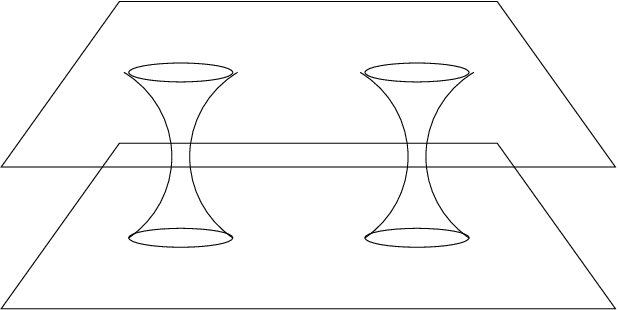
\includegraphics[height=40mm]{/home/runner/work/einsteintoolkit/einsteintoolkit/arrangements/EinsteinInitialData/IDAnalyticBH/doc/misner}
  \caption{The topology of the Misner spacetime is that of a pair of
  asymptotically flat sheets connected by a number of Einstein-Rosen
  bridges. By construction, an exact isometry exists between the upper
  and lower sheet across the throats. The parameter $\mu_0$ is a
  measure of the distance of a loop in the surface, passing through
  one throat and out the other.}
\end{figure}

Two implementations of the Misner data are available. The first of
these, ``\texttt{misner\_bh}'', is due to Joan Masso, Ed Seidel and
Karen Camarda, and implements the original two-throat solution. The
more general solution was implemented by Steve Brandt and Carsten
Gundlach, and is available as ``\texttt{multiple\_misner\_bh}''.

\subsection{Two-throat Misner data}

The \texttt{misner\_bh} initial data generates a metric of the form
\begin{equation}
  ds^2 = -dt^2 + \psi^4 (dx^2 + dy^2 + dz^2),
\end{equation}
where the conformal factor $\psi$ is given by
\begin{equation}
  \psi = \sum^N_{n=-N}
  \frac{1}{\sinh(\mu_0 n)}
  \frac{1}{\sqrt{x^2 + y^2 + (z + \coth(\mu_0 n))^2}}.
\end{equation}
The extrinsic curvature for the Misner data is zero.

The parameter $\mu_0$ is a measure of the ratio of mass to separation
of the throats, and is set using the parameter
\texttt{idanalyticbh::mu}. For values less than $\mu\simeq 1.8$, the
throats will have a single event horizon.

The summation limit $N$ can be set using the parameter
\texttt{idanalyticbh::nmax}. Ideally, it should tend to infinity, but
in practice the default value of $N=30$ works well enough for the
applications that have been tested. The \texttt{misner\_nbh} parameter
is only used for the \texttt{multiple\_misner\_bh} multi-throat data,
and will be ignored for the \texttt{misner\_bh} initial data, which
assumes two throats.

For the given metric, the ADM mass of the system is determined via
\begin{equation}
  m = 4 \sum^N_{n=1} \frac{1}{\sinh(\mu_0 n)}.
\end{equation}
This quantity is determined automatically and written to standard
output.

If the conformal form of the metric is used (via the
\texttt{admbase::metric\_type} parameter), then derivatives of the
conformal factor are computed analytically from the derivatives of the
above expression for $\psi$.

To make use of the two black hole initial data, a variation of the
following set of parameters can be used:
\begin{verbatim}
  ActiveThorns = "... ADMBase StaticConformal IDAnalyticBH ..."

  admbase::metric_type = "static conformal"

  admbase::initial_data = "misner_bh"
  idanalyticbh::mu = 2.2
\end{verbatim}


\section{Multiple-throat Misner data}

The generalisation of the above form of data to multiple black holes
is available as the \texttt{multiple\_misner\_bh} initial data set. The
conformal factor is determined by recursively applying a Misner
isometry condition to each of the black holes relative to the others.

The black holes are arranged at equal-spaced angles on a circle around
the origin in the $xy$-plane. The radius of the circle is $\coth\mu_0$,
where $\mu_0$ is given by the \texttt{idanalyticbh::mu} parameter, and
the first black hole lies on the $x$-axis (as in Figure
\ref{fig:multi_misner}).
\begin{figure}
  \centering
  \label{fig:multi_misner}
  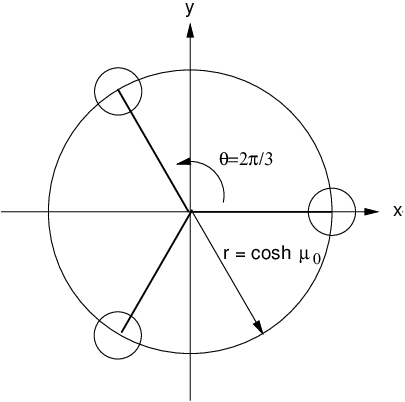
\includegraphics[height=40mm]{/home/runner/work/einsteintoolkit/einsteintoolkit/arrangements/EinsteinInitialData/IDAnalyticBH/doc/multi_misner}
  \caption{Configuration for three Misner throats using the
  \texttt{multiple\_misner\_bh} initial data.}
\end{figure}

The number of throats is given by the parameter
\texttt{idanalyticbh::misner\_nbh}, which defaults to 1 and has a
hard-coded upper limit of 10. The number of terms used in the Misner
expansion is controlled by the parameter
\texttt{idanalyticbh::nmax}, which has a default value of 30.

For this version of the Misner data, derivatives of the conformal
factor $\psi$ are determined numerically by finite differencing,
using values of $\psi$ calculated at small distances from the point at
which the derivative is to be evaluated. The size of the numerical
stencil is hardcoded at $dx=10^-6$.

As an example, a parameter file implementing 3 Misner black holes on a
circle of radius $\cosh 4$ would use the following parameters:
\begin{verbatim}
  ActiveThorns = "... ADMBase StaticConformal IDAnalyticBH ..."

  admbase::metric_type = "static conformal"

  admbase::initial_data = "multiple_misner_bh"

  idanalyticbh::misner_nbh = 3
  idanalyticbh::mu = 4
\end{verbatim}


\section{Brill-Lindquist}

The Brill-Lindquist initial data is an alternate form of multi-throat
data which differs from the Misner data mainly in its choice of
spacetime topology. Whereas the Misner data presumes that the throats
connect a pair of asymptotically flat spacetimes which are identical
to each other, the Brill-Lindquist data connects each throat to a
separate asymptotically flat region \cite{CactusEinstein_IDAnalyticBH_brill-lindquist:1963}.
\begin{figure}
  \centering
  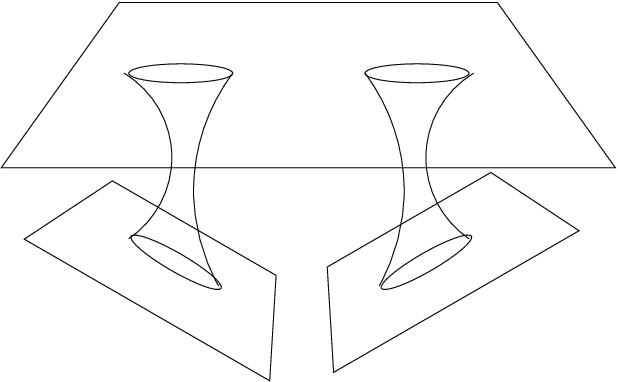
\includegraphics[height=40mm]{/home/runner/work/einsteintoolkit/einsteintoolkit/arrangements/EinsteinInitialData/IDAnalyticBH/doc/brill_lindquist}
  \caption{Two Brill-Lindquist throats connecting separate
    asymptotically flat regions.}
\end{figure}
The form of the conformal factor is:
\begin{equation}
  \psi = 1 + \sum_{i=1}^N \frac{m_i}{2r_i},
\end{equation}
where the $m_i$ and $r_i$ are the masses and positions of the $i$
particles.

The parameter specifying the number of black holes is
\texttt{idanalyticbh::bl\_nbh}. A maximum of four black holes can be
specified. The mass and $(x,y,z)$ position of the first black hole is
given by \texttt{bl\_M\_1}, \texttt{bl\_x0\_1}, \texttt{bl\_y0\_1},
\texttt{bl\_z0\_1}, with corresponding parameters for the second to
fourth black holes. Note that the default values for each of the
position coordinates are $0.0$, so that only the coordinates off
of the axes must be specified.

If the conformal metric is used, then derivatives of the conformal
factor are calculated from the analytic derivatives of the above
expression for the conformal factor.

To initialise a run with a pair of Brill-Lindquist black holes with
masses $1$ and $2$ and located at $\pm 1$ on the $y$-axis, a set of
parameters such as the following could be used:
\begin{verbatim}
  ActiveThorns = "... ADMBase StaticConformal IDAnalyticBH ..."

  admbase::metric_type = "static conformal"

  admbase::initial_data = "bl_bh"

  idanalyticbh::bl_nbh = 2

  idanalyticbh::bl_M_1 = 1.0
  idanalyticbh::bl_y0_1 = 1.0

  idanalyticbh::bl_M_2 = 2.0
  idanalyticbh::bl_y0_2 = -1.0
\end{verbatim}

\begin{thebibliography}{9}
  \bibitem{CactusEinstein_IDAnalyticBH_mtw-isotropic}
    See, for instance, p. 840 of:
    Misner, C. W., Thorne, K. S., and Wheeler, J. A. (1973)
    \emph{Gravitation}, W. H. Freeman, San Francisco.
  \bibitem{CactusEinstein_IDAnalyticBH_brandt-seidel:1996}
    Brandt, Steven R. and Seidel, Edward (1996)
    \emph{Evolution of distorted rotating black holes. III. Initial
    data},
    Phys. Rev., \textbf{D54}, 1403--1416.
  \bibitem{CactusEinstein_IDAnalyticBH_misner:1960}
    Misner, Charles W. (1960)
    \emph{Wormhole Initial Conditions},
    Phys. Rev., \textbf{118}, 1110--1111.
  \bibitem{CactusEinstein_IDAnalyticBH_misner:1963}
    Misner, Charles W. (1963)
    \emph{The Method of Images in Geometrostatics},
    Ann. Phys., \textbf{24}, 102--117.
  \bibitem{CactusEinstein_IDAnalyticBH_brill-lindquist:1963}
    Brill, Dieter R., and Lindquist, Richard W. (1963)
    \emph{Interaction Energy in Geometrostatics}
    Phys. Rev., \textbf{131}, 471--476.
\end{thebibliography}

% Do not delete next line
% END CACTUS THORNGUIDE



\section{Parameters} 


\parskip = 0pt

\setlength{\tableWidth}{160mm}

\setlength{\paraWidth}{\tableWidth}
\setlength{\descWidth}{\tableWidth}
\settowidth{\maxVarWidth}{multiple\_misner\_bh}

\addtolength{\paraWidth}{-\maxVarWidth}
\addtolength{\paraWidth}{-\columnsep}
\addtolength{\paraWidth}{-\columnsep}
\addtolength{\paraWidth}{-\columnsep}

\addtolength{\descWidth}{-\columnsep}
\addtolength{\descWidth}{-\columnsep}
\addtolength{\descWidth}{-\columnsep}
\noindent \begin{tabular*}{\tableWidth}{|c|l@{\extracolsep{\fill}}r|}
\hline
\multicolumn{1}{|p{\maxVarWidth}}{a\_kerr} & {\bf Scope:} private & REAL \\\hline
\multicolumn{3}{|p{\descWidth}|}{{\bf Description:}   {\em Angular momentum parameter of black hole}} \\
\hline{\bf Range} & &  {\bf Default:} 0.1 \\\multicolumn{1}{|p{\maxVarWidth}|}{\centering -1:1} & \multicolumn{2}{p{\paraWidth}|}{Between +1 and -1} \\\hline
\end{tabular*}

\vspace{0.5cm}\noindent \begin{tabular*}{\tableWidth}{|c|l@{\extracolsep{\fill}}r|}
\hline
\multicolumn{1}{|p{\maxVarWidth}}{bl\_m\_1} & {\bf Scope:} private & REAL \\\hline
\multicolumn{3}{|p{\descWidth}|}{{\bf Description:}   {\em Mass of 1st BL hole}} \\
\hline{\bf Range} & &  {\bf Default:} 1.0 \\\multicolumn{1}{|p{\maxVarWidth}|}{\centering :} & \multicolumn{2}{p{\paraWidth}|}{Anything} \\\hline
\end{tabular*}

\vspace{0.5cm}\noindent \begin{tabular*}{\tableWidth}{|c|l@{\extracolsep{\fill}}r|}
\hline
\multicolumn{1}{|p{\maxVarWidth}}{bl\_m\_2} & {\bf Scope:} private & REAL \\\hline
\multicolumn{3}{|p{\descWidth}|}{{\bf Description:}   {\em Mass of 2nd BL hole}} \\
\hline{\bf Range} & &  {\bf Default:} 1.0 \\\multicolumn{1}{|p{\maxVarWidth}|}{\centering :} & \multicolumn{2}{p{\paraWidth}|}{Anything} \\\hline
\end{tabular*}

\vspace{0.5cm}\noindent \begin{tabular*}{\tableWidth}{|c|l@{\extracolsep{\fill}}r|}
\hline
\multicolumn{1}{|p{\maxVarWidth}}{bl\_m\_3} & {\bf Scope:} private & REAL \\\hline
\multicolumn{3}{|p{\descWidth}|}{{\bf Description:}   {\em Mass of 3rd BL hole}} \\
\hline{\bf Range} & &  {\bf Default:} 1.0 \\\multicolumn{1}{|p{\maxVarWidth}|}{\centering :} & \multicolumn{2}{p{\paraWidth}|}{Anything} \\\hline
\end{tabular*}

\vspace{0.5cm}\noindent \begin{tabular*}{\tableWidth}{|c|l@{\extracolsep{\fill}}r|}
\hline
\multicolumn{1}{|p{\maxVarWidth}}{bl\_m\_4} & {\bf Scope:} private & REAL \\\hline
\multicolumn{3}{|p{\descWidth}|}{{\bf Description:}   {\em Mass of 4th BL hole}} \\
\hline{\bf Range} & &  {\bf Default:} 1.0 \\\multicolumn{1}{|p{\maxVarWidth}|}{\centering :} & \multicolumn{2}{p{\paraWidth}|}{Anything} \\\hline
\end{tabular*}

\vspace{0.5cm}\noindent \begin{tabular*}{\tableWidth}{|c|l@{\extracolsep{\fill}}r|}
\hline
\multicolumn{1}{|p{\maxVarWidth}}{bl\_nbh} & {\bf Scope:} private & INT \\\hline
\multicolumn{3}{|p{\descWidth}|}{{\bf Description:}   {\em Number of Brill Lindquist black holes}} \\
\hline{\bf Range} & &  {\bf Default:} 1 \\\multicolumn{1}{|p{\maxVarWidth}|}{\centering 1:4} & \multicolumn{2}{p{\paraWidth}|}{Between one and four holes implemented} \\\hline
\end{tabular*}

\vspace{0.5cm}\noindent \begin{tabular*}{\tableWidth}{|c|l@{\extracolsep{\fill}}r|}
\hline
\multicolumn{1}{|p{\maxVarWidth}}{bl\_x0\_1} & {\bf Scope:} private & REAL \\\hline
\multicolumn{3}{|p{\descWidth}|}{{\bf Description:}   {\em x-position of 1st BL hole}} \\
\hline{\bf Range} & &  {\bf Default:} 0.0 \\\multicolumn{1}{|p{\maxVarWidth}|}{\centering :} & \multicolumn{2}{p{\paraWidth}|}{Anything} \\\hline
\end{tabular*}

\vspace{0.5cm}\noindent \begin{tabular*}{\tableWidth}{|c|l@{\extracolsep{\fill}}r|}
\hline
\multicolumn{1}{|p{\maxVarWidth}}{bl\_x0\_2} & {\bf Scope:} private & REAL \\\hline
\multicolumn{3}{|p{\descWidth}|}{{\bf Description:}   {\em x-position of 2nd BL hole}} \\
\hline{\bf Range} & &  {\bf Default:} 0.0 \\\multicolumn{1}{|p{\maxVarWidth}|}{\centering :} & \multicolumn{2}{p{\paraWidth}|}{Anything} \\\hline
\end{tabular*}

\vspace{0.5cm}\noindent \begin{tabular*}{\tableWidth}{|c|l@{\extracolsep{\fill}}r|}
\hline
\multicolumn{1}{|p{\maxVarWidth}}{bl\_x0\_3} & {\bf Scope:} private & REAL \\\hline
\multicolumn{3}{|p{\descWidth}|}{{\bf Description:}   {\em x-position of 3nd BL hole}} \\
\hline{\bf Range} & &  {\bf Default:} 0.0 \\\multicolumn{1}{|p{\maxVarWidth}|}{\centering :} & \multicolumn{2}{p{\paraWidth}|}{Anything} \\\hline
\end{tabular*}

\vspace{0.5cm}\noindent \begin{tabular*}{\tableWidth}{|c|l@{\extracolsep{\fill}}r|}
\hline
\multicolumn{1}{|p{\maxVarWidth}}{bl\_x0\_4} & {\bf Scope:} private & REAL \\\hline
\multicolumn{3}{|p{\descWidth}|}{{\bf Description:}   {\em x-position of 4th BL hole}} \\
\hline{\bf Range} & &  {\bf Default:} 0.0 \\\multicolumn{1}{|p{\maxVarWidth}|}{\centering :} & \multicolumn{2}{p{\paraWidth}|}{Anything} \\\hline
\end{tabular*}

\vspace{0.5cm}\noindent \begin{tabular*}{\tableWidth}{|c|l@{\extracolsep{\fill}}r|}
\hline
\multicolumn{1}{|p{\maxVarWidth}}{bl\_y0\_1} & {\bf Scope:} private & REAL \\\hline
\multicolumn{3}{|p{\descWidth}|}{{\bf Description:}   {\em y-position of 1st BL hole}} \\
\hline{\bf Range} & &  {\bf Default:} 0.0 \\\multicolumn{1}{|p{\maxVarWidth}|}{\centering :} & \multicolumn{2}{p{\paraWidth}|}{Anything} \\\hline
\end{tabular*}

\vspace{0.5cm}\noindent \begin{tabular*}{\tableWidth}{|c|l@{\extracolsep{\fill}}r|}
\hline
\multicolumn{1}{|p{\maxVarWidth}}{bl\_y0\_2} & {\bf Scope:} private & REAL \\\hline
\multicolumn{3}{|p{\descWidth}|}{{\bf Description:}   {\em y-position of 2nd BL hole}} \\
\hline{\bf Range} & &  {\bf Default:} 0.0 \\\multicolumn{1}{|p{\maxVarWidth}|}{\centering :} & \multicolumn{2}{p{\paraWidth}|}{Anything} \\\hline
\end{tabular*}

\vspace{0.5cm}\noindent \begin{tabular*}{\tableWidth}{|c|l@{\extracolsep{\fill}}r|}
\hline
\multicolumn{1}{|p{\maxVarWidth}}{bl\_y0\_3} & {\bf Scope:} private & REAL \\\hline
\multicolumn{3}{|p{\descWidth}|}{{\bf Description:}   {\em y-position of 3nd BL hole}} \\
\hline{\bf Range} & &  {\bf Default:} 0.0 \\\multicolumn{1}{|p{\maxVarWidth}|}{\centering :} & \multicolumn{2}{p{\paraWidth}|}{Anything} \\\hline
\end{tabular*}

\vspace{0.5cm}\noindent \begin{tabular*}{\tableWidth}{|c|l@{\extracolsep{\fill}}r|}
\hline
\multicolumn{1}{|p{\maxVarWidth}}{bl\_y0\_4} & {\bf Scope:} private & REAL \\\hline
\multicolumn{3}{|p{\descWidth}|}{{\bf Description:}   {\em y-position of 4th BL hole}} \\
\hline{\bf Range} & &  {\bf Default:} 0.0 \\\multicolumn{1}{|p{\maxVarWidth}|}{\centering :} & \multicolumn{2}{p{\paraWidth}|}{Anything} \\\hline
\end{tabular*}

\vspace{0.5cm}\noindent \begin{tabular*}{\tableWidth}{|c|l@{\extracolsep{\fill}}r|}
\hline
\multicolumn{1}{|p{\maxVarWidth}}{bl\_z0\_1} & {\bf Scope:} private & REAL \\\hline
\multicolumn{3}{|p{\descWidth}|}{{\bf Description:}   {\em z-position of 1st BL hole}} \\
\hline{\bf Range} & &  {\bf Default:} 0.0 \\\multicolumn{1}{|p{\maxVarWidth}|}{\centering :} & \multicolumn{2}{p{\paraWidth}|}{Anything} \\\hline
\end{tabular*}

\vspace{0.5cm}\noindent \begin{tabular*}{\tableWidth}{|c|l@{\extracolsep{\fill}}r|}
\hline
\multicolumn{1}{|p{\maxVarWidth}}{bl\_z0\_2} & {\bf Scope:} private & REAL \\\hline
\multicolumn{3}{|p{\descWidth}|}{{\bf Description:}   {\em z-position of 2nd BL hole}} \\
\hline{\bf Range} & &  {\bf Default:} 0.0 \\\multicolumn{1}{|p{\maxVarWidth}|}{\centering :} & \multicolumn{2}{p{\paraWidth}|}{Anything} \\\hline
\end{tabular*}

\vspace{0.5cm}\noindent \begin{tabular*}{\tableWidth}{|c|l@{\extracolsep{\fill}}r|}
\hline
\multicolumn{1}{|p{\maxVarWidth}}{bl\_z0\_3} & {\bf Scope:} private & REAL \\\hline
\multicolumn{3}{|p{\descWidth}|}{{\bf Description:}   {\em z-position of 3nd BL hole}} \\
\hline{\bf Range} & &  {\bf Default:} 0.0 \\\multicolumn{1}{|p{\maxVarWidth}|}{\centering :} & \multicolumn{2}{p{\paraWidth}|}{Anything} \\\hline
\end{tabular*}

\vspace{0.5cm}\noindent \begin{tabular*}{\tableWidth}{|c|l@{\extracolsep{\fill}}r|}
\hline
\multicolumn{1}{|p{\maxVarWidth}}{bl\_z0\_4} & {\bf Scope:} private & REAL \\\hline
\multicolumn{3}{|p{\descWidth}|}{{\bf Description:}   {\em z-position of 4th BL hole}} \\
\hline{\bf Range} & &  {\bf Default:} 0.0 \\\multicolumn{1}{|p{\maxVarWidth}|}{\centering :} & \multicolumn{2}{p{\paraWidth}|}{Anything} \\\hline
\end{tabular*}

\vspace{0.5cm}\noindent \begin{tabular*}{\tableWidth}{|c|l@{\extracolsep{\fill}}r|}
\hline
\multicolumn{1}{|p{\maxVarWidth}}{epsilon} & {\bf Scope:} private & REAL \\\hline
\multicolumn{3}{|p{\descWidth}|}{{\bf Description:}   {\em Fudge factor}} \\
\hline{\bf Range} & &  {\bf Default:} 1.e-16 \\\multicolumn{1}{|p{\maxVarWidth}|}{\centering 0.0:*} & \multicolumn{2}{p{\paraWidth}|}{} \\\hline
\end{tabular*}

\vspace{0.5cm}\noindent \begin{tabular*}{\tableWidth}{|c|l@{\extracolsep{\fill}}r|}
\hline
\multicolumn{1}{|p{\maxVarWidth}}{mass} & {\bf Scope:} private & REAL \\\hline
\multicolumn{3}{|p{\descWidth}|}{{\bf Description:}   {\em Mass of black hole}} \\
\hline{\bf Range} & &  {\bf Default:} 2.0 \\\multicolumn{1}{|p{\maxVarWidth}|}{\centering :} & \multicolumn{2}{p{\paraWidth}|}{Not sure if it can be negative or not} \\\hline
\end{tabular*}

\vspace{0.5cm}\noindent \begin{tabular*}{\tableWidth}{|c|l@{\extracolsep{\fill}}r|}
\hline
\multicolumn{1}{|p{\maxVarWidth}}{misner\_nbh} & {\bf Scope:} private & INT \\\hline
\multicolumn{3}{|p{\descWidth}|}{{\bf Description:}   {\em Number of Misner black holes}} \\
\hline{\bf Range} & &  {\bf Default:} 1 \\\multicolumn{1}{|p{\maxVarWidth}|}{\centering 1:10} & \multicolumn{2}{p{\paraWidth}|}{Not more than 10} \\\hline
\end{tabular*}

\vspace{0.5cm}\noindent \begin{tabular*}{\tableWidth}{|c|l@{\extracolsep{\fill}}r|}
\hline
\multicolumn{1}{|p{\maxVarWidth}}{mu} & {\bf Scope:} private & REAL \\\hline
\multicolumn{3}{|p{\descWidth}|}{{\bf Description:}   {\em Misner mu value}} \\
\hline{\bf Range} & &  {\bf Default:} 1.2 \\\multicolumn{1}{|p{\maxVarWidth}|}{\centering 0:} & \multicolumn{2}{p{\paraWidth}|}{Non-negative} \\\hline
\end{tabular*}

\vspace{0.5cm}\noindent \begin{tabular*}{\tableWidth}{|c|l@{\extracolsep{\fill}}r|}
\hline
\multicolumn{1}{|p{\maxVarWidth}}{nmax} & {\bf Scope:} private & INT \\\hline
\multicolumn{3}{|p{\descWidth}|}{{\bf Description:}   {\em Number of terms to include for Misner series}} \\
\hline{\bf Range} & &  {\bf Default:} 30 \\\multicolumn{1}{|p{\maxVarWidth}|}{\centering 0:} & \multicolumn{2}{p{\paraWidth}|}{Non-negative} \\\hline
\end{tabular*}

\vspace{0.5cm}\noindent \begin{tabular*}{\tableWidth}{|c|l@{\extracolsep{\fill}}r|}
\hline
\multicolumn{1}{|p{\maxVarWidth}}{conformal\_storage} & {\bf Scope:} shared from STATICCONFORMAL & KEYWORD \\\hline
\end{tabular*}

\vspace{0.5cm}\parskip = 10pt 

\section{Interfaces} 


\parskip = 0pt

\vspace{3mm} \subsection*{General}

\noindent {\bf Implements}: 

idanalyticbh
\vspace{2mm}

\noindent {\bf Inherits}: 

admbase

staticconformal

grid
\vspace{2mm}

\vspace{5mm}\parskip = 10pt 

\section{Schedule} 


\parskip = 0pt


\noindent This section lists all the variables which are assigned storage by thorn EinsteinInitialData/IDAnalyticBH.  Storage can either last for the duration of the run ({\bf Always} means that if this thorn is activated storage will be assigned, {\bf Conditional} means that if this thorn is activated storage will be assigned for the duration of the run if some condition is met), or can be turned on for the duration of a schedule function.


\subsection*{Storage}NONE
\subsection*{Scheduled Functions}
\vspace{5mm}

\noindent {\bf CCTK\_PARAMCHECK}   (conditional) 

\hspace{5mm} idanalyticbh\_paramchecker 

\hspace{5mm}{\it construct parameters for analytic black hole solutions } 


\hspace{5mm}

 \begin{tabular*}{160mm}{cll} 
~ & Language:  & c \\ 
~ & Options:  & global \\ 
~ & Type:  & function \\ 
\end{tabular*} 


\vspace{5mm}

\noindent {\bf ADMBase\_InitialData}   (conditional) 

\hspace{5mm} schwarzschild 

\hspace{5mm}{\it construct initial data for a single schwarzschild black hole } 


\hspace{5mm}

 \begin{tabular*}{160mm}{cll} 
~ & Language:  & c \\ 
~ & Reads:  & grid::coordinates \\ 
~ & Storage:  & confac[1] \\ 
~ & Type:  & function \\ 
~ & Writes:  & staticconformal::conformal\_state(everywhere) \\ 
~& ~ &staticconformal::psi(everywhere)\\ 
~& ~ &staticconformal::confac\_1derivs(everywhere)\\ 
~& ~ &staticconformal::confac\_2derivs(everywhere)\\ 
~& ~ &admbase::metric(everywhere)\\ 
~& ~ &admbase::alp(everywhere)\\ 
~& ~ &admbase::curv(everywhere)\\ 
\end{tabular*} 


\vspace{5mm}

\noindent {\bf ADMBase\_InitialData}   (conditional) 

\hspace{5mm} kerrid 

\hspace{5mm}{\it construct initial data for a single kerr black hole } 


\hspace{5mm}

 \begin{tabular*}{160mm}{cll} 
~ & Language:  & c \\ 
~ & Reads:  & grid::x \\ 
~& ~ &grid::y\\ 
~& ~ &grid::z\\ 
~ & Storage:  & confac[1] \\ 
~ & Type:  & function \\ 
~ & Writes:  & staticconformal::conformal\_state(everywhere) \\ 
~& ~ &staticconformal::psi(everywhere)\\ 
~& ~ &staticconformal::confac\_1derivs(everywhere)\\ 
~& ~ &staticconformal::confac\_2derivs(everywhere)\\ 
~& ~ &admbase::metric(everywhere)\\ 
~& ~ &admbase::alp(everywhere)\\ 
~& ~ &admbase::curv(everywhere)\\ 
~& ~ &admbase::shift(everywhere)\\ 
\end{tabular*} 


\vspace{5mm}

\noindent {\bf ADMBase\_InitialData}   (conditional) 

\hspace{5mm} brilllindquist 

\hspace{5mm}{\it construct initial data for brill lindquist black holes } 


\hspace{5mm}

 \begin{tabular*}{160mm}{cll} 
~ & Language:  & c \\ 
~ & Reads:  & grid::x \\ 
~& ~ &grid::y\\ 
~& ~ &grid::z\\ 
~ & Storage:  & confac[1] \\ 
~ & Type:  & function \\ 
~ & Writes:  & staticconformal::conformal\_state(everywhere) \\ 
~& ~ &staticconformal::psi(everywhere)\\ 
~& ~ &staticconformal::confac\_1derivs(everywhere)\\ 
~& ~ &staticconformal::confac\_2derivs(everywhere)\\ 
~& ~ &admbase::metric(everywhere)\\ 
~& ~ &admbase::curv(everywhere)\\ 
\end{tabular*} 


\vspace{5mm}

\noindent {\bf ADMBase\_InitialData}   (conditional) 

\hspace{5mm} misner\_standard 

\hspace{5mm}{\it construct initial data for two misner black holes } 


\hspace{5mm}

 \begin{tabular*}{160mm}{cll} 
~ & Language:  & c \\ 
~ & Reads:  & grid::x \\ 
~& ~ &grid::y\\ 
~& ~ &grid::z\\ 
~ & Storage:  & confac[1] \\ 
~ & Type:  & function \\ 
~ & Writes:  & staticconformal::conformal\_state(everywhere) \\ 
~& ~ &staticconformal::psi(everywhere)\\ 
~& ~ &staticconformal::confac\_1derivs(everywhere)\\ 
~& ~ &staticconformal::confac\_2derivs(everywhere)\\ 
~& ~ &admbase::metric(everywhere)\\ 
~& ~ &admbase::curv(everywhere)\\ 
~& ~ &admbase::alp(everywhere)\\ 
\end{tabular*} 


\vspace{5mm}

\noindent {\bf ADMBase\_InitialData}   (conditional) 

\hspace{5mm} misner\_multiple 

\hspace{5mm}{\it construct initial data for multiple misner black holes } 


\hspace{5mm}

 \begin{tabular*}{160mm}{cll} 
~ & Language:  & c \\ 
~ & Reads:  & grid::x \\ 
~& ~ &grid::y\\ 
~& ~ &grid::z\\ 
~ & Storage:  & confac[1] \\ 
~ & Type:  & function \\ 
~ & Writes:  & staticconformal::conformal\_state(everywhere) \\ 
~& ~ &staticconformal::psi(everywhere)\\ 
~& ~ &staticconformal::confac\_1derivs(everywhere)\\ 
~& ~ &staticconformal::confac\_2derivs(everywhere)\\ 
~& ~ &admbase::metric(everywhere)\\ 
~& ~ &admbase::curv(everywhere)\\ 
\end{tabular*} 



\vspace{5mm}\parskip = 10pt 
\end{document}
